\section{Séquencement}
	\label{sec:sequencement}
	Pour établir notre planification, nous avons utilisé le logiciel MS Project. Les diagrammes ci-dessous tiennent compte des différents jalons qui ont été posés, soit imposés à tous dans les projets de 4INFO, soit définis nous-même.

	\subsection{Diagramme de Gantt}
		Le diagramme de Gantt visible sur la \ffigure{} \ref{fig:gantt} illustre le séquencement de notre projet. Les tâches ont été attribuées à une personne, et les durées ont été calculées pour une moyenne d'une heure de travail personnel par jour.

	\subsection{Planning des charges}
		Le planning de la \ffigure{} \ref{fig:planning_charge} illustre le cumul des heures de travail pour chaque personne. Nous avons essayé d'être homogènes dans la répartition des tâches de chacun.

		\begin{landscape}
		 	\begin{figure}
	            \centering
	            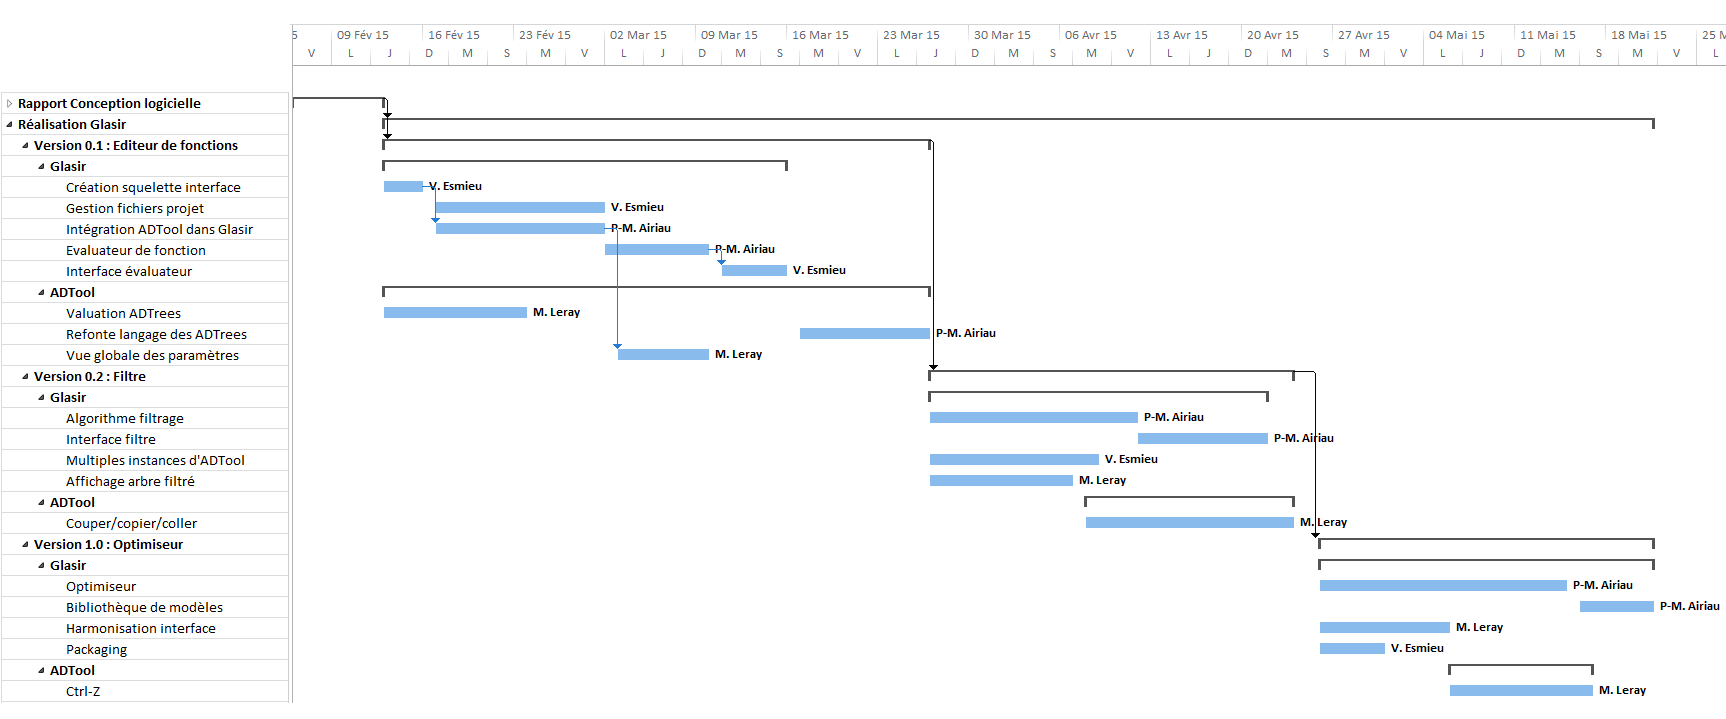
\includegraphics[height=0.70\textwidth]{figure/DiagGantt.png}
	            \caption{Diagramme de Gantt présentant la chronologie des tâches.}
	            \label{fig:gantt}
	        \end{figure}
	    \end{landscape}

		\begin{landscape}
		 	\begin{figure}
	            \centering
	            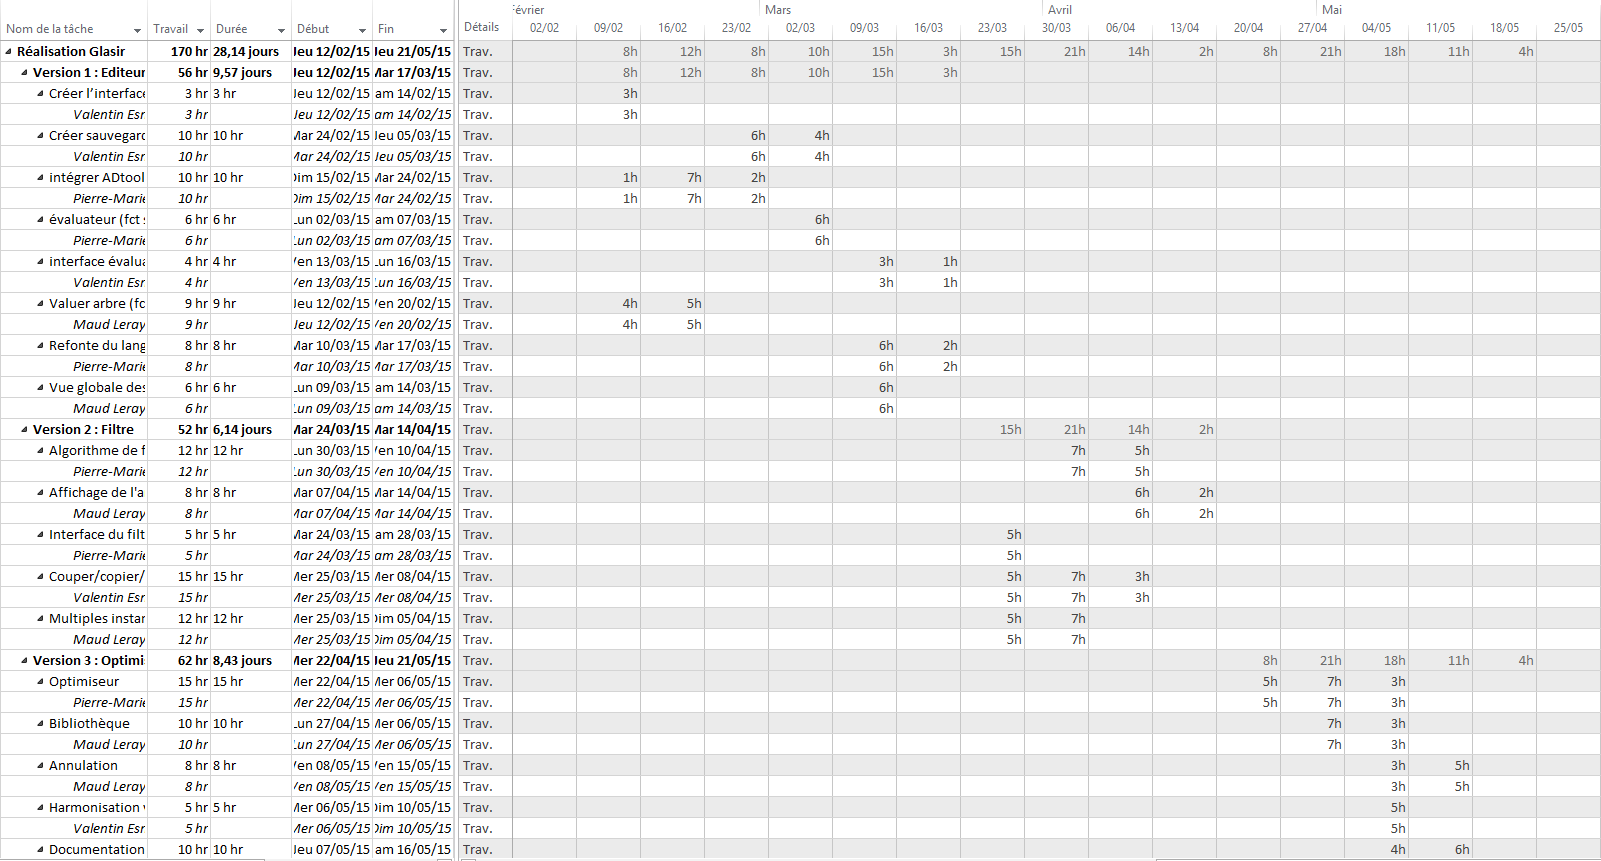
\includegraphics[height=0.70\textwidth]{figure/RepartitionTaches2.png}
	            \caption{Planning des charges réparties par personne}
	            \label{fig:planning_charge}
	        \end{figure}
	    \end{landscape}

	    \subsection{Utilisation des ressources}